\documentclass[11pt, leqno]{article}
\usepackage[utf8]{inputenc}
\usepackage{polski}
\usepackage{a4wide}

\usepackage{graphicx}
\usepackage{amsmath}
%\usepackage{bbm}
\usepackage{amsthm}
\usepackage{amssymb}
\usepackage{algorithmic}
\usepackage{ulsy}
\usepackage[usenames,dvipsnames]{color}
\usepackage{hyperref}
\hypersetup
{
    colorlinks=true,       	% false: boxed links; true: colored links
    linkcolor = OliveGreen,	% color of internal links
	 urlcolor = OliveGreen  	% color of external links
}
\newenvironment{Itemize}
{\begin{itemize}
  \setlength{\itemsep}{1pt}
  \setlength{\parskip}{0pt}
  \setlength{\parsep}{0pt}}
{\end{itemize}}

\title{Inverse Kinematics for Arm + Fingers Genetic Algorithm}
\date{\today}
\author{Marcin Januszkiewicz, Jakub Kowalski}


\begin{document}

\maketitle
\vspace{17em}
\tableofcontents
\newpage

\section{Sformułowanie zadania}
Zagadnienie kinematyki odwrotnej (\textit{ang.}\ inverse kinematics) dotyczy reprezentacji kończyn (ogólnie tzw.\ efektora) za pomocą geometrycznego modelu w którym kości estymowane są przez linie, natomiast stawom odpowiadają kąty. Zadaniem kinematyki odwrotnej jest znalezienie takich położeń stawów, dla których osiagana jest pożądana pozycja kończyny, np.\ zamocowana w pewnym punkcie startowym dosięga ona zadanego punktu końcowego. Możliwe położenia stawów określone są przez minimalny i maksymalny kąt rozwarcia. Chromosom jest to lista kątów odpowiadających rozwarciom kolejnych stawów kończyny.

Rozpatrywana przez nas rozszerzona wersja standardowego zagadnienia dotyczy kończyn o strukturze analogicznej do ręki, a mianowicie składających się z ciągu kości po którym następuje rozgałęzienie na kilka ciągów symulujących palce (rysunek \ref{fig:armf}.). Zadanie polega na znalezieniu ustawienia ręki w którym każdy palec dotyka innego punktu docelowego (punktów docelowych jest tyle samo co palców) a ręka nie koliduje z żadną znajdującą się na planszy przeszkodą.

\begin{figure}[h!]
	\centering
	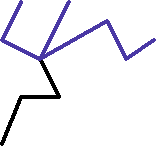
\includegraphics[scale=0.5]{armfingers}
	\caption{Kończyna o strukturze ręki: na czarno zaznaczone jest ramię, natomiast na niebiesko palce.}
	\label{fig:armf}
\end{figure}


\subsection{Format pliku wejściowego}
Scenariusz (plik zawierający informację o planszy oraz własciwościach ręki) jest plikiem o następującej konstrukcji (linie rozpoczynające się od \# traktowane są jako komentarz):
\begin{verbatim}
# Wielkość planszy w poziomie
10
# Wielkość planszy w pionie
5
# Punkt startowy (wszystkie punkty podane są w notacji X Y)
5 4
# Liczba punktów docelowych a tym samym liczba palców
2
# Punkty docelowe
1 1
9 1
# Liczba kości w ramieniu
2
# Specyfikacja ramienia, każda kość opisana jest za pomocą długości 
# oraz minimalnej i maksymalnej miary kąta stawu względem kości poprzedzającej
3 0 360
1 0 360
# W analogiczny sposób podawane są informacje o wszystkich palcach
# Liczba kości pierwszego palca
2
# Specyfikacja pierwszego palca
3 0 360
3 0 360
# Tak samo dla drugiego palca i kolejnych
2
3 0 360
3 0 360
# Liczba przeszkód
2
# Liczba punktów w pierwszej przeszkodzie
3
# Kolejne punkty pierwszej przeszkody
# Przeszkoda traktowana jest jako zbiór linii pomiędzy kolejnymi podanymi punktami
# aby przeszkoda tworzyła figurę zamknietą, ostatni punkt powinien być taki sam jak pierwszy
1 3
2 4
4 4
# Analogicznie wyspecyfikowana jest druga przeszkoda i dalsze
5
2 1
3 2
4 1
3 0
2 1
\end{verbatim}

\section{Obsługa programu}
Graficzny interfejs użytkownika, wykorzystywany przez program testowy, przedstawiony jest na rysunku \ref{fig:gui}.

\begin{figure}[h!]
	\centering
	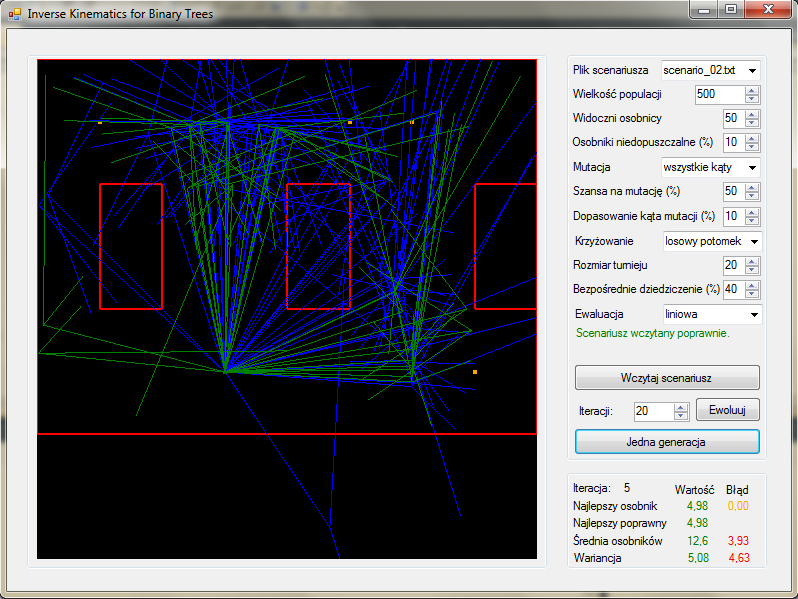
\includegraphics[scale=0.5]{gui}
	\caption{Interfejs programu}
	\label{fig:gui}
\end{figure}

Program pozwala wybrać jeden z przygotowanych plików scenariusza oraz określić podstawowe parametry ewolucji. Po wczytaniu scenariusza można uruchomić ewolucję na kilka pokoleń zgodnie z przekazanymi danymi (najpierw wykonywana jest zadana liczba ewolucji dla ramion a następnie dla palców) lub wyewoluować kolejną generację zajmując się całymi kończynami.

Statystyki aktualnej populacji pozwalają ocenić osobników (pokazywane są wartości błędu i minimalizowanej funkcji celu dla osobnika najlepszego w calej populacji, najlepszego bezbłędnego oraz wartości średnie), a także ocenić różnorodność i zbieżność populacji poprzez zmieniające się wartości wariancji (dla błędu oraz funkcji oceny) i oryginalności populacji (liczonej jako stosunek osobników bez duplikatów do liczebności populacji).

Wizualizacja przedstawia planszę zakodowaną w scenariuszu. Czerwone linie oznaczają przeszkody, zielony punkt jest punktem startowym, natomiast pomarańczowe punkty są punktami docelowymi. Czarne obszary są to miejsca nieosiągalne z punktu startowego, błękitne -- takie w których może znajdować się nadgarstek poprawnej kończyny. Na wizualizacji zaznaczeni są również najlepsi osobnicy. Niebieskie linie pokazują przebieg najlepszego osobnika w całej populacji, natomiast zielone najlepszego bezbłędnego (jeśli istnieje).

\section{Ewolucja}
Zastosowany algorytm ewolucyjny częściowo bazuje na algorytmie IDEA \cite{PFI}, jednak ze względu na specyfikę problemu zastosowane zostały rozwiązania dedykowane. W szczególności za najistotniejszy punkt kończyny uznaliśmy nadgarstek, w którym kończy się ramię a zaczynają palce. Rozpatrywanie umiejscowień nadgarstka pozwala rozbić problem dla całej ręki na podproblemy bardziej podobne do postawionych przez kinematykę odwrotną w standardowym jej sformułowaniu. 

\subsection{Heurystyki}
W celu wyznaczenia możliwych umiejscowień nadgarstka wykonywane są pewne heurystyczne obliczenia dla planszy podzielonej na odpowiednio małe partycje. Heurystyki te pozwalają na odnalezienie takich obszarów, z których można dosięgnąć palcami wszystkich punktów docelowych a ramieniem punktu startowego. Sprawdzana jest jedynie osiagalność w linii prostej, po wyznaczeniu dla każdej kończyny (biorąc pod uwagę możliwe rozwarcia stawów) jej maksymalnej i minimalnej długości. Heurystycznie, za pomocą algorytmu przeszukiwań, wyznaczana jest również osiągalność obszarów planszy od punktu startowego.


\subsection{Operatory ewolucyjne}

\begin{itemize}
	\item Mutacja polega na losowym zaburzeniu pojedynczych miar kątów.
	\item Selekcja odbywa się metodą turniejową z sumy mnogościowej populacji dzieci i rodziców.
	\item Krzyżowanie odbywa się pomiędzy parą rodziców, która generje parę potomków. Metoda krzyżowania zalezy od parametru nakierowującego ewolucję. Miary kątów są dziedziczone po rodzicach lub wyznaczane (dla pewnego losowego zaburzenie $\beta\in[0, 1]$ i rodziców $\alpha_1$, $\alpha_2$) za pomocą wzorów:
	\[
		\frac{\alpha_1 + \alpha_2 + \beta(\alpha_1 - \alpha_2)}{2} \quad\quad \frac{\alpha_1 + \alpha_2 + \beta(\alpha_2 - \alpha_1)}{2}
	\]
	\begin{itemize}
		\item jeżeli ewolucja jest nastawiona na modyfikację ramienia, to uśrednieniu ulegają wartości kątów ramienia a palce są dziedziczne po rodzicach,
		\item nakierowanie na ewolucję palców prowadzi do bezpośredniego dziedziczenia ramienia i modyfikacji kątów palców,
		\item opcja krzyżowania całościowego ewoluuje wszystkie stawy kończyny.
	\end{itemize}
\end{itemize}

\subsubsection{Funkcja celu}
Podstawą wartości funkcji jest dystans od punktu ramienia do celu, wyznaczany za pomocą dwóch metod: zwracania dystansu w linii prostej oraz obliczania drogi potrzebnej na obejście przeszkód z wyznaczonymi otoczkami wypukłymi. W obecnej wersji algorytmu, ze względu na szybkość obliczeń, wykorzystywana jest prostsza z napisanych funkcji.

Oprócz odległości do celu wyznaczana jest również miara niepoprawności osobnika, liczona jako liczba przecięć segmentów chromosomu z przeszkodami. Docelowo algorytm dąży do trzymania jedynie niewielkiej liczby osobników niepoprawnych, rokujących na uzyskanie dobrych potomków.

Sposób wyznaczania wartości funkcji celu zależy od nakierowania aktualnego kroku ewolucji. Nakierowanie na ewolucję ramienia sprawia, że ocena chromosomu zalezy od dystansu nadgarstka do najbliższego, wyznaczonego heurystycznie, obiecującego obszaru w którym mógłby się on znajdować. W takim wypadku nie są liczone błędy wynikające z niepoprawnego ułożenia palców a jedynie spowodowane przez kości ramienia. Z kolei ewolucja palców znajduje zachłannie dopasowanie palec--punkt docelowy i liczy dla tego dopasowania sumę odległości.


\section{Testy}

Algorytm był testowany na kilku przygotowanych scenariuszy i dla różnych wartości parametrów.

\subsection{Scenariusze testowe}
Stworzone zostały cztery scenariusze testowe, przedstawione na rysunkach \ref{fig:sc1}, \ref{fig:sc2}, \ref{fig:sc3}, \ref{fig:sc4} (scenariusz 1 różni się od scenariusza 2 dodatkową kością ramienia, co w widoczny sposób zwiększa manewrowość kończyny zmniejszając skuteczność heurystyki wyznaczającej możliwe pozycje nadgarstka).


\begin{figure}[h!]
	\centering
	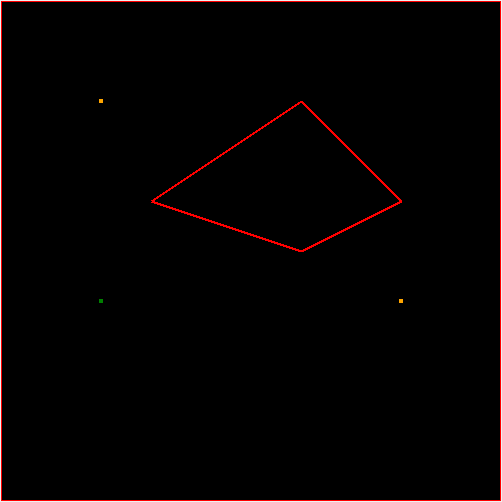
\includegraphics[scale=0.4]{scenario1}
	\caption{Scenariusz testowy 1}
	\label{fig:sc1}
\end{figure}

\begin{figure}[h!]
	\centering
	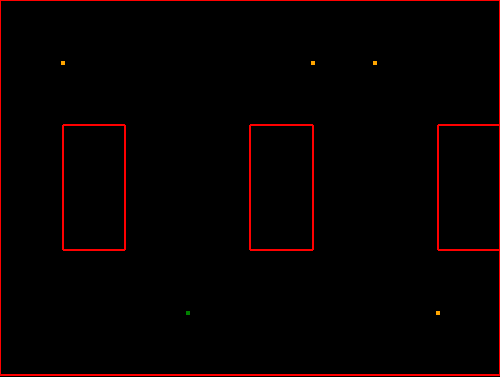
\includegraphics[scale=0.4]{scenario2}
	\caption{Scenariusz testowy 2}
	\label{fig:sc2}
\end{figure}

\begin{figure}[h!]
	\centering
	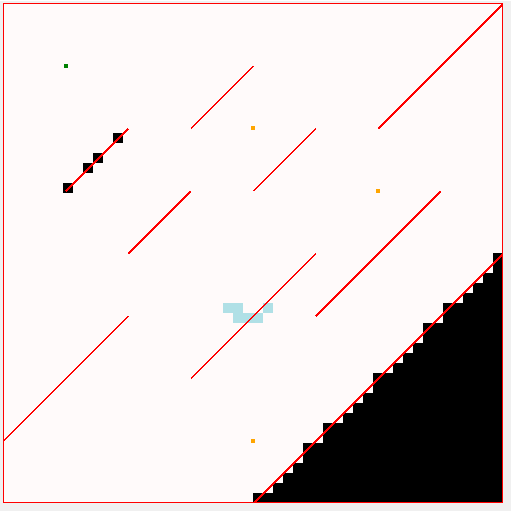
\includegraphics[scale=0.4]{scenario3}
	\caption{Scenariusz testowy 3}
	\label{fig:sc3}
\end{figure}

\begin{figure}[h!]
	\centering
	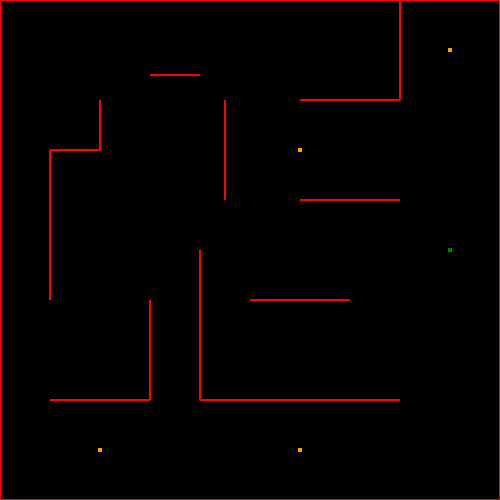
\includegraphics[scale=0.4]{scenario4}
	\caption{Scenariusz testowy 4}
	\label{fig:sc4}
\end{figure}


\subsection{Wyniki}
Osiągane wyniki nie są zadawalające ponieważ algorytm, pomimo sprawnego umiejscowienia nadgarstka i wyewoluowania osobników znajdujących się blisko celu, ma problem z osiągnięciem optymalnego rozwiązania. Dla nawet małej populacji (50 osobników) w scenariuszach testowych nadgarstek był obiecująco umieszczany w przeciągu pierwszych 10 -- 20 iteracji. Problem ze zbieżnością całego chromosomu wynika zapewne ze specyfiki zadania, które w szczególności nie określa odgórnie jaki palec ma zmierzać do jakiego celu. Powoduje to, że krzyżowanie osobników obierających różne dopasowania oddala populację od osiagnięcia rozwiązania.

\section{Podsumowanie}
Podsumowując, rozszerzenie dziedziny zadania poskutkowało znacznym jego utrudnieniem. Różnicę tę widać na przykładzie szybkości osiagania połowicznego celu jakim jest umiejscowienie nadgarstka. Aby podobne rezultaty osiągać dla całego osobnika, należałoby rozbudować chromosom przechowując w nim informację o najbardziej obiecującym przypasowaniu palców do punktów docelowych. Wiązałoby się to również z modyfikacją operacji krzyżowania tak aby przekazywała również informację o dopasowaniu palców.

Warto zwrócić także uwagę na aspekty obliczeniowe związane z problemami geometrycznymi. Zarówno wyznaczenie początkowych heurystyk, jak i obliczanie funkcji dystansu oraz błędu wymagają sprawdzania dużej liczby warunków, co przenosi ciężar obliczeń z ewolucji właściwej na aspekty dodatkowe i pozwala na wyewoluowanie w sensownym czasie mniejszej liczby generacji na mniejszych populacjach osobników.

Ponadto, w rozwiązaniach zauważone zostały również pewne artefakty (znikanie osobników dopuszczalnych, pogarszanie najlepszych rozwiązań), które mogą wskazywać na błąd w implementacji.

Warto zwrócić uwagę, że inne metody liczenia odległości (chodzenie po figurze lub jej otoczce wypukłej) powodowały bardzo duże spowolnienie nawet dla niewiekich domyślnych parametrów programu.  

Bez rozwiązania kwestii optymalizacji tych metod korzystanie z nich na większych planszach lub dla większego rozmiaru populacji byłoby niepraktyczne.

\begin{thebibliography}{1}
	\bibitem{PFI} Patryk Filipiak, {\it Optymalizacja ewolucyjna z predykcją w dynamicznym problemie kinematyki odwrotnej}. Wrocław, Seminarium ZMN IIUWr 2011.
\end{thebibliography}


\end{document}